\chapter{NP-Completeness}

\section{SAT Cont.}

\begin{definition}
    A Boolean formula \(\phi\) is in \underline{Conjunctive Normal Form} (CNF) if it has the form
    \[
        \phi = (x \lor \bar{y} \lor z) \land (\bar{x} \lor \bar{s} \lor z \lor u) \land \cdots \land (\bar{z} \lor \bar{u})
    \]

    \textbf{Literal} : a variable or a negated variable

    \textbf{Clause}: an OR of literals (the thing in a brace)
    
    \textbf{CNF}: an AND of clauses(all of them).
    
    \textbf{3CNF}: a CNF with exactly 3 literals in each clause 

    \(3SAT\) = \{ \(\langle \phi \rangle | \phi\) is a staisfiable 3CNF formula\} 
\end{definition}

\begin{definition}
    A \(k-clique\) in a graph is a subset of \(k\) nodes all directly connected by edges.   

    \begin{example}
        \begin{figure}[H]
            \centering
            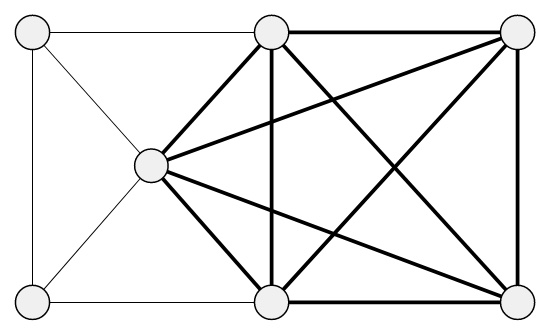
\includegraphics[width=0.6\textwidth]{f7.23.jpg}
            \caption{A graph with a 5-CLIQUE}
        \end{figure}
    \end{example}

    \(CLIQUE\) = \{\(\langle G, k \rangle\) | graph G contains k-clique\} 
\end{definition}

We will show \(3SAT \leq_P CLIQUE\) 

\begin{theorem}
    \(3SAT \leq_P CLIQUE\) 
\end{theorem}
\begin{proof}
    IDEA: \(\phi\) is satisfiable \(\iff\) \(G\) has a \(k-clique\)        

    Construction to make the transformation from \(3SAT\) to \(k-CLIQUE\):
    \begin{remark}[Transformation]
        Here is the mapping from CNF to the graph:
        \begin{itemize}
            \item \(3SAT \; literal \mapsto \) vertex (node) in \(k-CLIQUE\)   
            \item \(3SAT \; \#clause \mapsto\) \(k\) in \(k-CLIQUE\)   
            \item \(3SAT\) be TRUE at same time \(\mapsto\) edges in the graph
        \end{itemize}

        Principle in making edges:
        \begin{enumerate}
            \item can't make edges within a clause
            \item can't make inconsistent edges (for example we can't connect \(a\) with \(\bar{a}\))
        \end{enumerate}

        This is what the transformation looks like, forbidden edges are connected in red line:
        \begin{figure}[H]
            \centering
            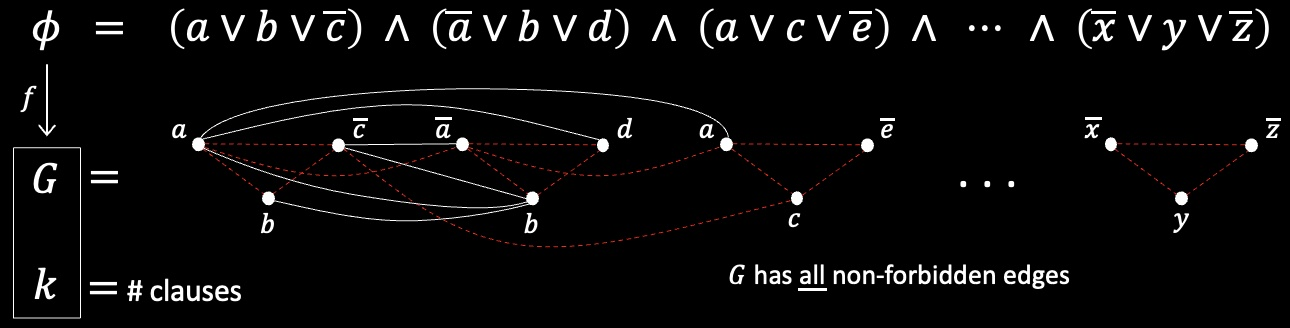
\includegraphics[width=\textwidth]{l15.1.jpg}
            \caption{transformation from CNF to graph}
        \end{figure}
    \end{remark}

    \begin{lemma}[Forward]
        \(\phi\) is satisfiable \(\implies\) \(G\) has a \(k-clique\).   
    \end{lemma}
    \begin{proof}
        Take any satisfying assignment to \(\phi\). Pick 1 true literal in each clause. 

        The corresponding nodes in \(G\) are a \(k-clique\) because they don't have forbidden edges.  
    \end{proof}

    \begin{lemma}[Backward]
        \(G\) has a \(k-clique\) \(\implies\) \(phi\) is satisfiable.
    \end{lemma}
    \begin{proof}
        Take any \(k-clique\) in \(G\), it must have 1 node in each clause.  

        Set each corresponding literal TRUE. That gives a satisfying assignment to \(\phi\). 
    \end{proof}

    Notice that the reduction (transformation) \(f\) is computable in polynomial time. 
\end{proof}

\begin{corollary}
    \(CLIQUE \in P \implies 3SAT \in P\) 
\end{corollary}

\begin{remark}
    Does the theorem require 3 literals per clause?

    The answer is no, it works for any size clause.
\end{remark}


\section{NP-Completeness}

\begin{definition}
    Language \(B\) is  \underline{NP-Complete}  if
    \begin{enumerate}
        \item \(B \in NP\) 
        \item For all \(A \in NP\), \(A \leq_P B\)  
    \end{enumerate}

    \begin{remark}
        \begin{definition}[NP-hard]
            A problem is \textbf{NP-hard} if all problems in NP are polynomial time reducible to it, even though it may not be in NP itself.  
        \end{definition}

        Notice that the 2nd constraint for defining \(B\) is NP-complete is actually saying \(B\) is NP-hard.  

        So we can say a language is NP-complete if it is in NP, and it is NP-hard.
    \end{remark}
\end{definition}


If \(B\) is NP-complete and \(B \in P\) then P = NP. 

\begin{theorem}[Cook-Levin Theorem]
    \(SAT\) is NP-complete 
\end{theorem}
\begin{proof}
    Next lecture. Assume it is true for now.
\end{proof}

\begin{note}
    \(\forall A \in NP\):
    \[
        A \leq_P SAT \leq_P 3SAT \leq_P CLIQUE/HAMPATH
    \]
\end{note}

\begin{note}
    To show some language \(C\) is NP-complete, show \(3SAT \leq_P C\). 
\end{note}


\textbf{Importance of NP-complete}:
\begin{enumerate}
    \item Showing \(B\) is NP-complete is evidence of computational intractability.
    (Show a problem is NP-complete is a powerful evidence that it is not P)
    \item Gives a good candidate for proving \(P \neq NP\).  
\end{enumerate} 

\begin{theorem}
    \(HAMPATH\) is NP-complete. 
\end{theorem}
\begin{proof}
    Show \(3SAT \leq_P HAMPATH\) (assume 3SAT is NP-Complete) 

    The simulation is so hard to describe, but this is a famous question, so I will just describe the setup here:

    \textbf{Transformation of each variable/literal \(x_i\)}: it is represented with a diamond-shaped structure that contains a horizontal row of nodes:
    \begin{figure}[H]
        \centering
        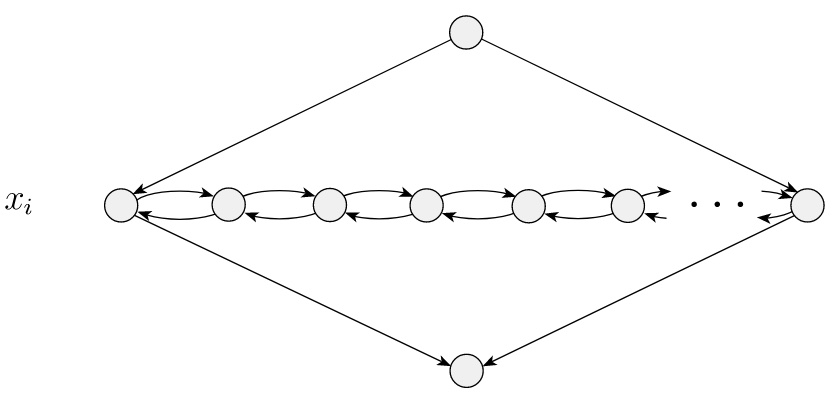
\includegraphics[width=0.6\textwidth]{f7.47.jpg}
    \end{figure}

    \textbf{Transformation of each clause \(c_j\)}: as a node. 

    \textbf{Global structure}:
    \begin{figure}[H]
        \centering
        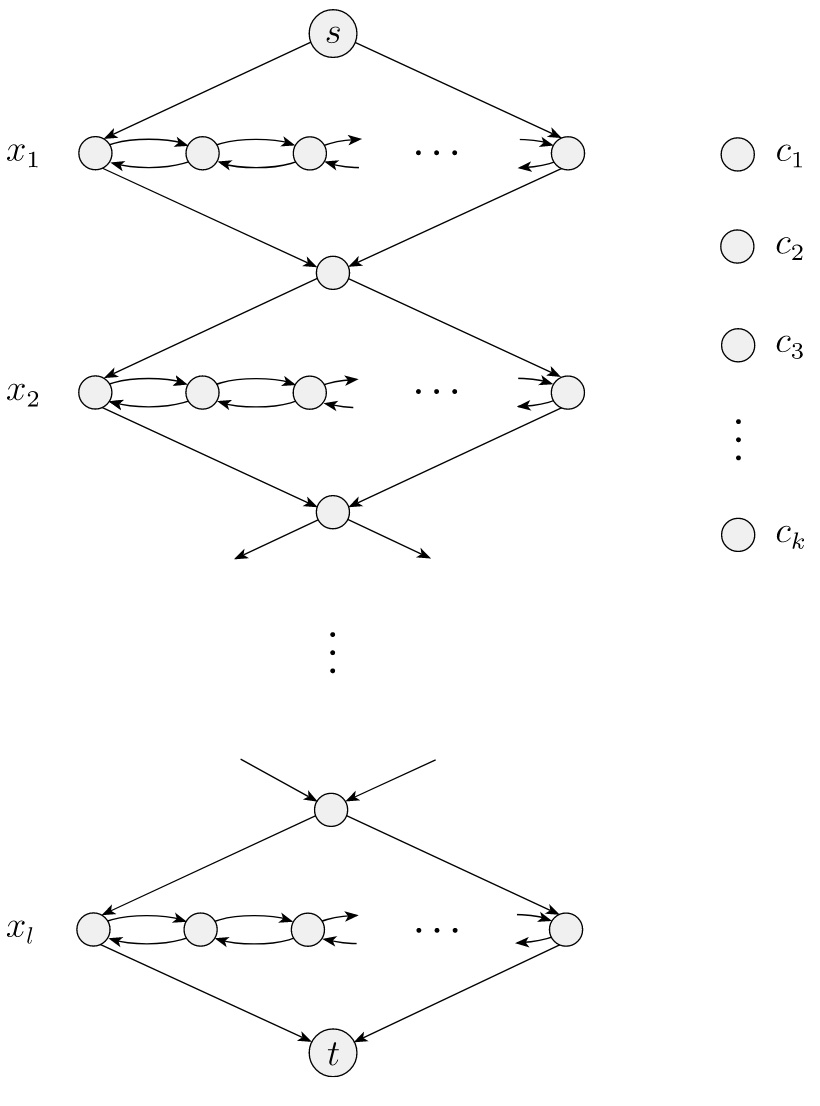
\includegraphics[width=0.6\textwidth]{f7.49.jpg}
    \end{figure}

    The core is the representation of a clause \(c_j\) contains an \(x_i\) or \(\bar{x_i}\):
    \begin{figure}[H]
        \begin{minipage}{0.48\textwidth}
            \centering
            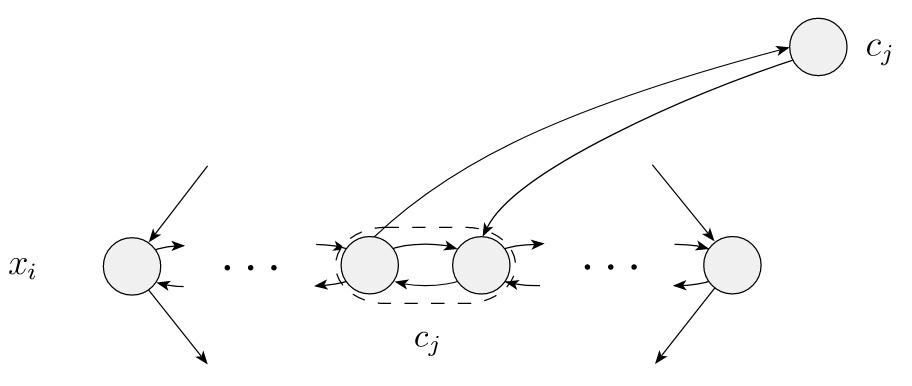
\includegraphics[width=\linewidth]{f7.51.jpg}
            \caption{the additional edges when \(c_j\) contains \(x_i\) }
        \end{minipage}\hfill
        \begin{minipage}{0.48\textwidth}
            \centering
            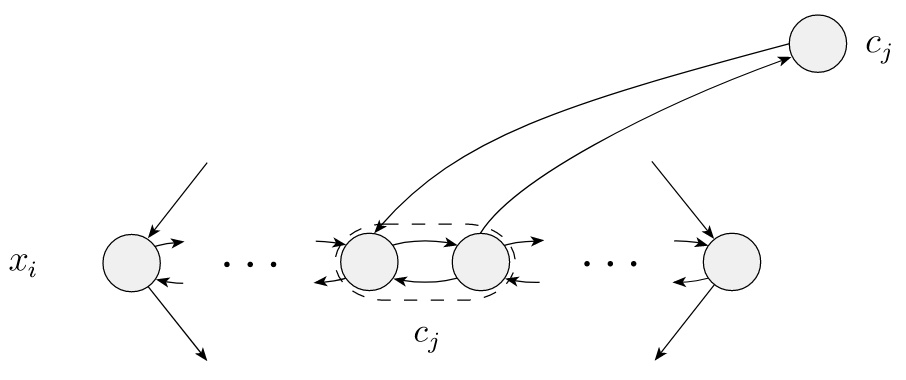
\includegraphics[width=\linewidth]{f7.52.jpg}
            \caption{the additional edges when \(c_j\) contains \(\bar{x_i}\) }
        \end{minipage}
    \end{figure}

    (The complete proof can be easily got from internet.)
\end{proof}

\begin{remark}
    Would this construction show the undirected Hamilton path problem is NP-complete?

    No, the construction depends on \(G\) being directed. 
\end{remark}

\section{Summary}
How to do polynomial reduction.